\documentclass[11pt]{article}
\usepackage{naaclhlt2012}
\usepackage{times}
\usepackage{latexsym}
\usepackage{url}
\usepackage{graphicx}
\usepackage{subfig}
\usepackage{amsmath}
\usepackage{array}
\usepackage{multirow}
\usepackage{rotating}


% \author{Juri Ganitkevitch, Benjamin Van Durme \and
%   Chris Callison-Burch \\
%   Department of Computer Science, Johns Hopkins University \\
%   Baltimore, MD 21218, USA}

\author{}

\title{Monolingual Distributional Similarity for Text-to-Text Generation}

\begin{document}
\maketitle

\begin{abstract}
  Previous work obtained collections of paraphrases by either relying
  on bilingual parallel datasets, or by using distributional
  similarity metrics over large text corpora. Our approach combines
  these two orthogonal sources of information and directly integrates
  them into the our paraphrasing system's log-linear model. We compare
  different distributional similarity feature sets and show
  significant improvements in output quality on the example
  text-to-text generation task of sentence compression, beating two
  state-of-the-art baselines.
\end{abstract}

\section{Introduction}

A wide variety of applications in natural language processing can be
cast in terms of text-to-text generation. Given input in the form of
natural language, a text-to-text generation system produces natural
language output that fulfills previously defined constraints and
objectives on both the text's surface form and meaning. Paraphrases,
i.e.\ differing textual realizations of the same meaning, are a
crucial components of text-to-text generation systems, and have been
successfully applied to tasks such as multi-document summarization
\cite{Barzilay1999,BarzilayThesis}, query expansion
\cite{Anick1999,Riezler2007}, question answering
\cite{mckeown:1979:ACL,Ravichandran2002}, sentence compression and
simplification.

One way of using paraphrases for text-to-text generation is to
appropriate the machinery developed for statistical machine
translation \cite{Quirk2004}. Syntactically informed machine
translation approaches have been used to create sentential
paraphrasing systems. Both \newcite{Cohn2008} and
\newcite{Ganitkevitch2011} described large-scale extraction methods
for syntactically annotated paraphrases from bilingual parallel
corpora. This framework can be adapted to many sentential text-to-text
generation tasks.

In this paper, we describe an extension of
\newcite{Ganitkevitch2011}'s approach by introducing a new component
into the paraphrasing system that is \emph{not} derived from the
statistical machine translation machinery. We use an orthogonal source
of information: monolingual distributional similarity. More
specifically, we show that:
\begin{itemize}
\item Using monolingual distributional similarity features improves
  paraphrase quality beyond what we can achieve with features estimated
  from bilingual data. 

\item Different types of monolingual distributional information can be
  used to achieve improvements in grammaticality or word sense
  disambiguation.

\item We define distributional similarity for paraphrase patterns that
  contain gaps, e.g.  \vspace{-6pt}
  \begin{equation*}\mathit{sim}(\text{one }\mathit{JJ}\text{ instance
      of }\mathit{NP}, \text{a }\mathit{JJ}\text{ case of }\mathit{NP}
    ).  \vspace{-2pt}
  \end{equation*} 
  This generalizes over \newcite{Chan2011} which defined the notion
  for contiguous phrases or single-word gaps.

\item Finally, we compare our method to several strong baselines on
  the text-to-text generation task of sentence compression. Our method
  beats a purely bilingually sourced paraphrasing system and an
  ILP-based compression model.
\end{itemize}

\section{Background}

\subsection{Paraphrase Extraction via Pivoting}
\label{sec-scfgs}

\begin{figure}[!t]
\begin{center}
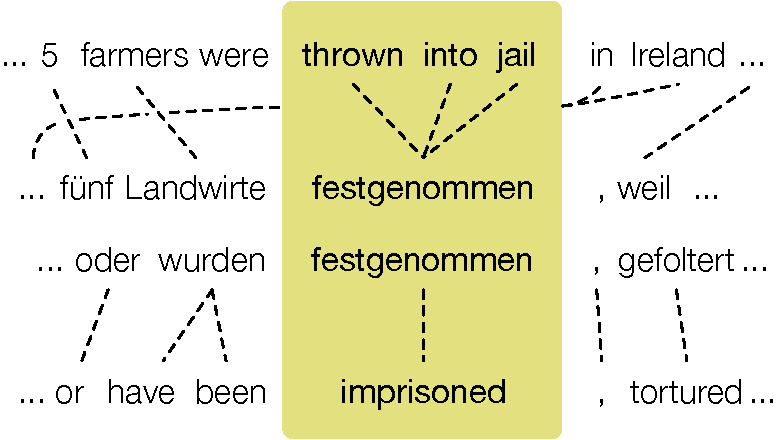
\includegraphics[width=0.9\linewidth]{figures/phrasal_pivoting.pdf}
\end{center}
\caption{Pivot-based paraphrase extraction for contiguous phrases. Two
phrases translating to the same phrase in the foreign language are
assumed to be paraphrases of one another.}
\label{fig-example-compression}
\end{figure}


\begin{figure}[!t]
\begin{center}
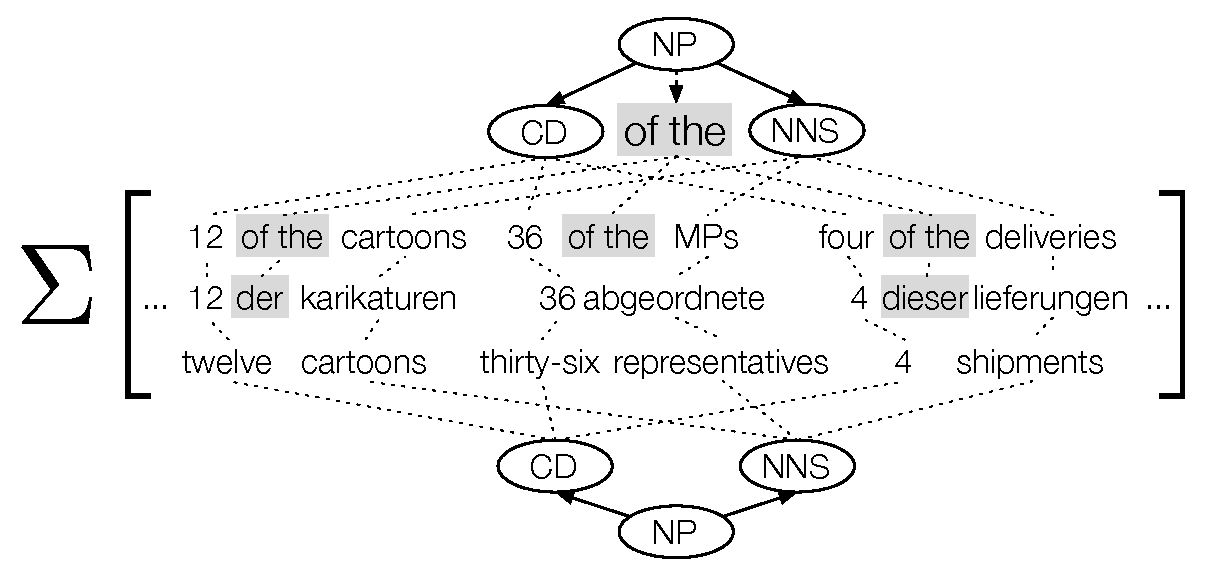
\includegraphics[width=0.99\linewidth]{figures/syntactic_pivoting.pdf}
\end{center}
\caption{An example of syntactic paraphrase extraction via the
  pivoting approach. We sum over the multiple surface forms that give
  rise to the syntactic pattern.}\label{fig-syntactic-pivoting}
\end{figure}

Following \newcite{Ganitkevitch2011}, we formulate our paraphrases as
a syntactically annotated \emph{ synchronous context-free grammar}
(SCFG) \cite{Aho1972,Chiang2005}.  An SCFG rule has the form:
\begin{equation*}
  \mathbf{r} = C \rightarrow \langle f, e, \sim, \vec{\varphi} \rangle ,
\end{equation*}
where the left-hand side of the rule, $C$, is a nonterminal and the
right-hand sides $f$ and $e$ are strings of terminal and nonterminal
symbols with an equal number of nonterminals. The function $\sim$
defines a one-to-one correspondency function between the nonterminals
in $f$ and $e$. Drawing on machine translation terminology, we refer
to $f$ as the \emph{source} and $e$ as the \emph{target}
side of the rule.

Each rule is annotated with a vector of feature functions
$\vec{\varphi} = \{\varphi_1 ... \varphi_N \}$ that, using a
corresponding weight vector $\vec{\lambda}$, are combined in a
log-linear model to compute the \emph{cost} of applying $\mathbf{r}$:
\begin{equation}
  \mathit{cost}(\mathbf{r}) = -\sum_{i=1}^N \lambda_i \log \varphi_i .
\end{equation}
A wide variety of feature functions can be formulated. We detail the
feature set used in our experiments in Sections~\ref{distributional-similarity-model} and \ref{sec-setup}.

\begin{figure}[!t]
\begin{center}
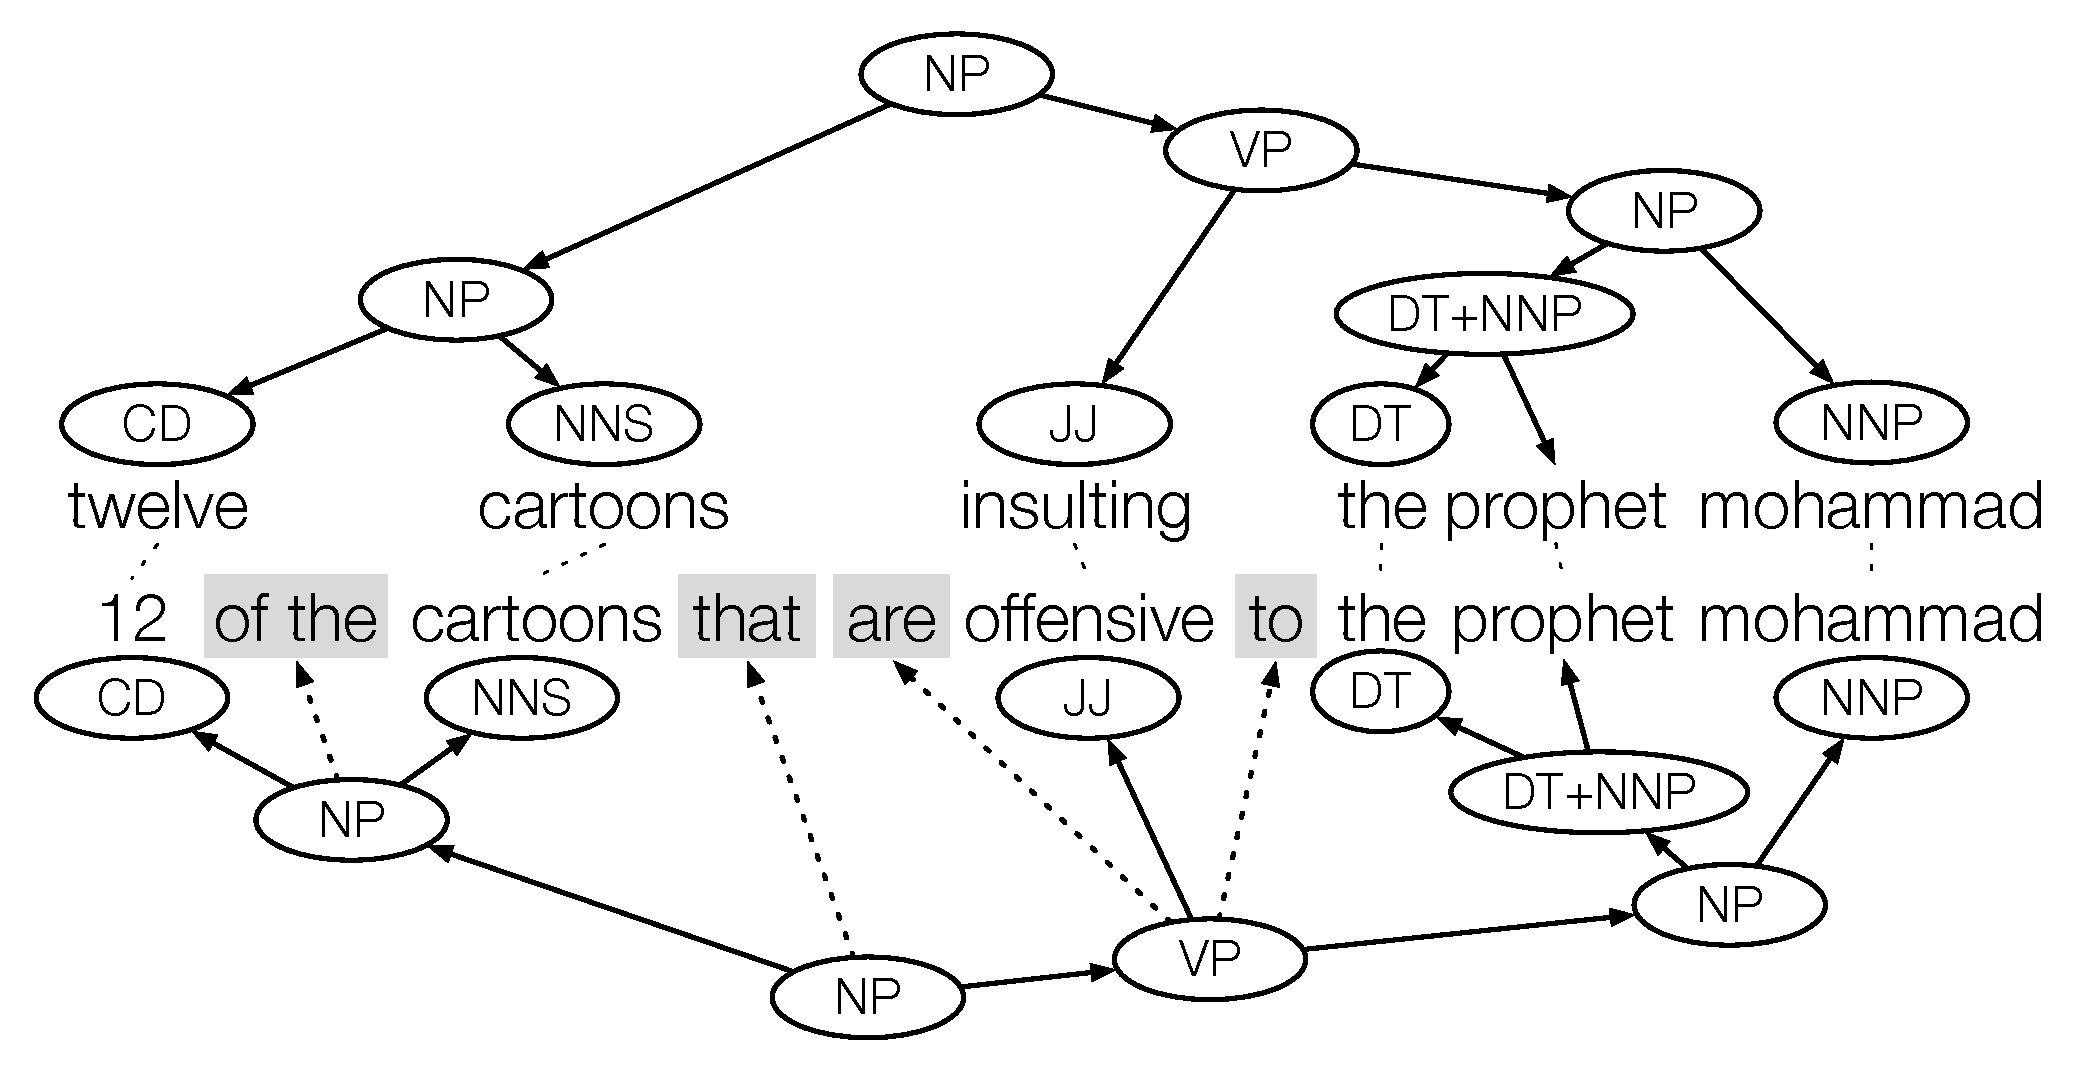
\includegraphics[width=0.99\linewidth]{figures/example_compression.pdf}
\end{center}
\caption{An example of a synchronous paraphrastic derivation, here a
  sentence compression. Shaded words are deleted in the indicated rule
  applications.}
\label{fig-example-compression}
\end{figure}

To obtain a paraphrase grammar, we first extract a translation grammar
that translates a foreign language into English. Then, for each pair
of translation rules where the left-hand side $C$ and foreign string
$f$ match:
\begin{eqnarray*}
    \mathbf{r}_1 = C \rightarrow \langle f, e_1, \sim_1, \vec{\varphi}_1
  \rangle \phantom{,} \\
  \mathbf{r}_2 = C \rightarrow \langle f, e_2, \sim_2, \vec{\varphi}_2
  \rangle ,
\end{eqnarray*}
we use the intuition that two English strings $e_1$ and $e_2$ that
translate to the same foreign string $f$ are equivalent in meaning,
and \emph{pivot} over $f$ to create a paraphrase rule
\cite{Ganitkevitch2011,Callison-Burch2008,Callison-Burch2005}:
\begin{equation*}
  \mathbf{r}_p = C \rightarrow \langle e_1, e_2, \sim_p, \vec{\varphi}_p \rangle ,
\end{equation*}
with a combined nonterminal correspondency function $\sim_p$.
Similarly, the paraphrase feature vector $\vec{\varphi}_p$ is computed
from the translation feature vectors $\vec{\varphi}_1$ and
$\vec{\varphi}_2$ by following the pivoting idea. For instance, we
estimate the conditional paraphrase probability $p(e_2 | e_1)$ by
marginalizing over all shared foreign-language translations $f$:
\begin{eqnarray}
  p(e_2|e_1) &=& \sum_f p(e_2,f|e_1)\\
  &=& \sum_f p(e_2|f,e_1) p(f|e_1) \\
  &\approx& \sum_f p(e_2|f) p(f|e_1) .
\label{eq-paraphrase-probability}
\end{eqnarray}
Figure~\ref{fig-syntactic-pivoting} illustrates syntax-constrained
pivoting and feature aggregation over multiple foreign language
translations for a paraphrase pattern. After the SCFG has been
extracted, it can be straightforwardly used within the normal machine
translation machinery.  Figure~\ref{fig-example-compression} shows an
example for a synchronous paraphrastic derivation produced as a result
of applying our grammar in the decoding process.

The approach we outlined in this section relies on aligned bilingual
texts to identify phrases and patterns that are equivalent in
meaning. When extracting paraphrases from monolingual text, we have to
rely on an entirely different set of semantic cues and features.

\subsection{Monolingual Distributional Similarity}
\label{sec-mds}

Paraphrase extraction from monolingual corpora measures the similarity
of phrases based on contextual features. To describe a phrase $e$, we
define a set of features that describe the context of an occurrence of
$e$ in our corpus. The resulting feature vectors $\vec{s}_{e,i}$ are
aggregated over all occurrences of $e$, resulting in a
\emph{distributional} signature for $e$, $\vec{s}_e = \sum_i
\vec{s}_{e,i}$.  Following the intuition that phrases with similar
meanings occur in similar contexts, we can then identify $e'$ as a
paraphrase of $e$ by computing the cosine similarity between their
distributional signatures:
\begin{equation*}
  \mathit{sim}(e, e') = \frac{\vec{s}_e \cdot \vec{s}_{e'}}{|\vec{s}_e||\vec{s}_{e'}|}.
\end{equation*}

A wide variety of features have been used to describe the
distributional context of a phrase. Rich, linguistically informed
feature sets that relie on dependency and constituency parses,
part-of-speech tags, or lemmatization have been proposed early on
\cite{ChurchHanks91,Lin2001}. For instance, in \newcite{Lin2001}'s
work, a phrase is described by the various syntactic relations it has
with lexical items in its context, such as: ``for what verbs do we see
with the phrase as the subject?'', or ``what adjectives modify the
phrase?''

However, when moving to vast text collections or collapsed
representations of large text corpora, linguistic annotations can
become impractically expensive to produce. A straightforward and
widely used solution is to fall back onto lexical $n$-gram features,
i.e.  ``what words or bigrams have we seen to the left of this
phrase?'' A substantial body of work has focussed on using this type
of features for a variety of purposes in NLP and text-to-text
generation.
\cite{LapataKellerSaLP05,Bhagat2008,LinEtAlLREC10,VanDurmeLallACL10}.

%In this work, we will qualitatively and quantitatively compare the two approaches to distributional signature construction. Section~\ref{sec-ranking} discusses the difference in effects on paraphrase ranking, and Section~\ref{sec-results} presents human evaluation results on a text-to-text task.



\subsection{Additional Related Work}

In a GEMS workshop paper, \newcite{Chan2011} presented an initial investigation into combining phrasal
paraphrases obtained through bilingual pivoting with monolingual
distributional information. They presented a re-ranking approach and
evaluated their method via a substitution task. We expand on their by
both substantially generalizing the formalism used, and by applying an
evaluating our paraphrase system on a text-to-text generation task.


\section{Incorporating Distributional Similarity}
\label{sec-scoring}

In order to incorporate the distributional similarity information into
the paraphrasing system, we need to calculate similarity scores for
the paraphrastic SCFG rules in our grammar. For rules with purely
lexical right-hand sides $\bar{e}_1$ and $\bar{e}_2$ this is a simple
task, and the similarity score $\mathit{sim}(\bar{e}_1, \bar{e}_2)$
can be included in the rule's feature vector $\vec{\varphi}$. For
rules whose right-hand sides contain gaps, computing a similarity
score is less straightforward.

Figure~\ref{fig-pattern-scoring} shows an example of a discontinuous
rule and illustrates our solution: we decompose the discontinuous
patterns that make up the right-hand sides of a rule $\mathbf{r}$ into
pairs of contiguous phrases $\mathcal{P}(\mathbf{r}) = (\bar{e},
\bar{e}')$, for which we can look up distributional signatures and
compute similarity scores. This decomposition into phrases is
non-trivial, since our sentential paraphrase rules often involve
significant reordering or structural changes. To avoid comparing
unrelated phrase pairs, we require $\mathcal{P}(\mathbf{r})$ to be
consistent with a token alignment $\mathbf{a}$. We define and compute
$\mathbf{a}$ analogously to the word alignments used in statistical
machine translation.

\begin{figure}[!t]
\begin{center}
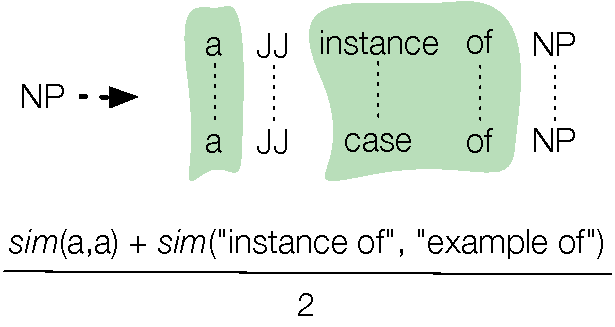
\includegraphics[width=0.85\linewidth]{figures/pattern_scoring.pdf}
\end{center}
\caption{Scoring a rule by extracting and scoring contiguous phrases
  consistent with the alignment. The overall score of the rule is
  determined by}\label{fig-pattern-scoring}
\end{figure}

We define the overall similarity score of the rule to be the average
of the similarity scores of all extracted phrase pairs:
\begin{equation*}
  \mathit{sim}(\mathbf{r}, \mathbf{a}) = \frac{1}{|\mathcal{P}(\mathbf{a})|}
  \sum_{(e, e') \in \mathcal{P}(\mathbf{a})}\mathit{sim}(e, e') .
\end{equation*}
Since the distributional signatures for long, rare phrases may be
computed from only a handful of occurrences, we additionally query for
the shorter sub-phrases that are more likely to have been observed
often enough for reliable signature and thus similarity estimates. The
intended sparsity-reduction is similar to the backing-off concept in
statistical $n$-gram language modeling.

Our two similarity scores are incorporated into the paraphraser as an
additional rule feature $\varphi_{\mathit{sim}}$. The corresponding
weight $\lambda_{\mathit{sim}}$ is estimated along with the other
$\lambda_i$ in our training framework, detailed in
Section~\ref{sec-setup}.


\section{Paraphrase Ranking}
\label{sec-ranking}

\begin{table*}[!t]
\begin{center}
\begin{tabular}{|cr|cr|cr|}
  \hline
  \multicolumn{6}{|c|}{\emph{ADJP/NP} $\rightarrow$ \emph{ADJP/VP}
    assume that \emph{S/NP}} \\
  \hline
  \multicolumn{2}{|c|}{Pivot-Based} &
  \multicolumn{2}{c|}{$n$-gram} &
  \multicolumn{2}{c|}{Rich} \\
  \hline

  \ldots cause \ldots & 8.88 &
  \ldots allow \ldots & 4.02 &
  \ldots imagine \ldots & 1.99 \\

  \ldots show \ldots & 8.93 &
  \ldots find \ldots & 4.77 &
  \ldots show \ldots & 2.05 \\

  \ldots is \ldots & 9.04 &
  \ldots make \ldots & 4.81 &
  \ldots to make \ldots & 2.23 \\

  \ldots make \ldots & 9.11 &
  \ldots enable \ldots & 4.89 &
  \ldots cause \ldots & 2.35 \\

  \ldots imagine \ldots & 9.11 &
  \ldots have \ldots & 5.06 &
  \ldots say \ldots & 2.42 \\

  \hline
  \multicolumn{6}{c}{} \\
  \hline
  \multicolumn{6}{|c|}{\emph{NP/PP} $\rightarrow$ \emph{DT}
    sign of \emph{NP/PP}} \\
  \hline
  \multicolumn{2}{|c|}{Pivot-Based} &
  \multicolumn{2}{c|}{$n$-gram} &
  \multicolumn{2}{c|}{Rich} \\
  \hline


  \ldots with \ldots & 10.25 &
  \ldots of \ldots & 4.10 &
  \ldots view to \ldots & 2.08 \\

  \ldots view to \ldots & 10.67 &
  \ldots with \ldots & 5.50 &
  \ldots attempt at \ldots & 2.19 \\

  \ldots attempt at \ldots & 10.80 &
  \ldots expression of \ldots & 6.40 &
  \ldots body of \ldots & 2.46 \\


  \ldots face of \ldots & 10.82 &
  \ldots setting of \ldots & 6.63 &
  \ldots face of \ldots & 2.46 \\

  \ldots talk about \ldots & 10.95 &
  \ldots provision of \ldots & 6.72 &
  \ldots talk about \ldots & 2.58 \\

  \hline
\end{tabular}
\end{center}
\normalsize
\caption{Comparison of top 5 paraphrase rankings for two example patterns in
  our grammar. The top row shows the left-hand side and source side of
  the rule. The nonterminal symbols on the target side are identical
  to the source side in all cases and are omitted for legibility. The
  numbers next to the paraphrase candidates are the log-linear model
  costs, i.e. lower is better\footnote{The log-linear model costs are
    only comparable within each column.}}
\label{tab-ranking}
\end{table*}

Finding good estimates of the quality of a paraphrase pair is crucial
to the usefulness of a paraphrase system in practice. The key
motivation to this work is that by combining information from both
pivoted and monolingual distributional similarity-based paraphrases we
can the quality of our system beyond either individual approach.

To test our hypothesis, we empirically analyze the effects the
incorporation of distributional similarity has on the ranking of
paraphrases within our grammar. In this section, we contrast the
pivoting-based baseline system, with the integrations of the two
previously described distributional similarity models: simple unigram
features trained on a large $n$-gram corpus (which we will refer to as
the ``$n$-gram'' model), and a similarity model with a richer feature
set (dubbed ``rich''), but which has lower coverage.

The ranking of paraphrase candidates is crucially dependent on the
log-linear model weights $\lambda_i$. To make our analysis realistic,
we adopt the feature weights produced by our tuning approach (see
Section~\ref{sec-setup}). In our rank calculation, we omit all
compression-oriented features (such as word and character counts
etc.), as well as the identity rule feature. This is done so that our
ranking comparison is based on general paraphrase quality rather than
task-specific utility.

Table~\ref{tab-ranking} shows two example patterns pulled from our
grammar, along with the top 5 paraphrases according to each system. We
see a number of high-ranking bad paraphrases such as \emph{assume
  that} going to \emph{is} or \emph{sign of} paraphrasing as
\emph{with} that occur in the baseline system. These seem to be the
result of errors in word alignment, and only in fringe cases would
they result in grammatical or meaning-preserving output. While the
$n$-gram model partially fixes the issue, it is limited by its unigram
feature set, making it prone to errors such as reducing \emph{sign of}
to \emph{of}. Again, the rich model fares significantly better here,
mostly eliminating bad paraphrases in favor of true, and occasionally
interesting paraphrases such as \emph{imagine} for \emph{assume that}.

These qualitative observations suggest that a rich feature set is indeed valuable
when integrating distributional similarity information into a
pivot-based paraphrasing system. In next section, we quantify
this gain by evaluating our system on a text-to-text generation
problem.



\section{Experimental Setup}
\label{sec-setup}

\subsection{Task: Sentence Compression}

To evaluate our method on a real text-to-text application, we chose to
adopt the setting and datasets from \cite{Ganitkevitch2011}. We train
our paraphrasing system to produce sentence level compression by way
of sentential paraphrasing. We contrast our distributional
similarity-informed paraphrase system with an uninformed pivoting-only
(but otherwise identical) baseline, as well as an implementation of
\newcite{Clarke2008}'s state-of-the-art compression model which uses a
series of constraints in an integer linear programming (ILP)
solver.

\subsection{Baseline Paraphrase Grammar}

We extracted our paraphrase grammar from the French--English portion
of the Europarl corpus (version 5) \cite{koehn2005europarl}. The
Berkeley aligner and the Berkeley parser were used to align the bitext
and parse the English side, respectively. The paraphrase grammar was
produced using the Hadoop-based Thrax grammar extractor's paraphrase
mode. The syntactic nonterminal labels we allowed in the grammar were
limited to constituent labels and CCG-style slashed
categories. Paraphrase grammars extracted via pivoting tend to grow
very large. To keep the grammar size manageable, we pruned away all
paraphrase rules whose phrasal paraphrase probabilities $p(e_1|e_2)$
or $p(e_2|e_1)$ were smaller than $0.001$.

We extended the feature set used by \newcite{Ganitkevitch2011} with a
number of features that aim to better describe a rule's compressive
power: on top of the word count features $c_{\mathit{src}}$ and
$c_{\mathit{tgt}}$ and the word count difference feature
$c_{\mathit{diff}}$, we add character based count and difference
features $\mathit{char}_{\mathit{src}}$,
$\mathit{char}_{\mathit{tgt}}$, and $\mathit{char}_{\mathit{diff}}$,
as well as log-compression ratio features $c_{\mathit{cr}} = \log
\frac{c_{\mathit{tgt}}}{c_{\mathit{src}}}$ and the analogously defined
$\mathit{char}_{\mathit{cr}}$.

For model tuning and decoding, we used the Joshua machine translation
system \cite{Joshua-3.0}. The model weights were estimated using an
implementation of the PRO tuning algorithm \cite{PRO2011}, with
\textsc{Pr\'ecis} as our objective function \cite{Ganitkevitch2011}.  The
language model used in our paraphraser and the \newcite{Clarke2008}
baseline system is a Kneser-Ney discounted 5-gram model estimated on
the Gigaword corpus using the SRILM toolkit \cite{SRILM}.


\subsection{Distributional Similarity Model}\label{distributional-similarity-model}
In order to investigate the impact of the feature set used, we chose
to extract two collections of distributional similarity-based
paraphrases. Using a web-scale $n$-gram corpus
\cite{GoogleNgrams,LinEtAlLREC10}, we extract unigram features for the
words to the left and right for phrases up to a length of 4. The
features are weighed with the $n$-gram count given by the dataset. The
resulting collection comprised context vectors for the 200 million
most frequent 1- to 4-grams in the dataset.

For contrast, we use the constituency- and dependency-parsed Los
Angeles Times/Washington Post portion of the Gigaword corpus
\cite{Gigaword}. The following feature set is used to compute phrase
contexts over this dataset:
\begin{itemize}
\item Lexical and part-of-speech unigram and bigram features,
  drawn from a three-word window to the right and left of the phrase. 
\item Features based on dependencies for both links into and out of
  the phrase, labeled with the corresponding lexical item and POS. If
  the phrase is syntactically well-formed we additionally include
  lexical and POS features for its head.
\item Syntactic features for constituents governing the phrase, as
  well as for CCG-style slashed constituent labels for the phrase,
  split by governing constituent and missing constituent. 
\end{itemize}
Figure~\ref{fig-rich-context} illustrates our choice of feature
set. As a result we obtain context information for over 12 million 1-
to 4-gram phrases.

\begin{figure}[!t]
\begin{center}
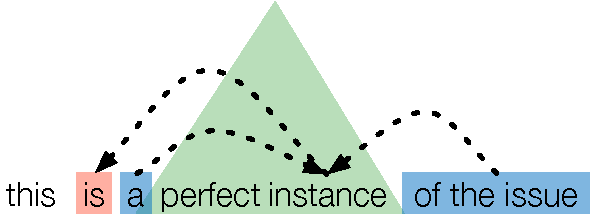
\includegraphics[width=0.99\linewidth]{figures/rich_context.pdf}
\end{center}
\caption{An example of word-labeled dependency-based rich
  distributional features over a parsed text corpus. The phrase
  ``perfect instance'' is annotated with the in- and outgoing
  dependency links, the words at the end of the links and a
  count.}\label{fig-rich-context}
\end{figure}

Much like \newcite{Ravichandran2005} and \newcite{Bhagat2008}, we
relied on Locality Sensitive Hashing (LSH), to make the use of these
large collections practical. In order to avoid explicitly computing
the feature vectors, which can be memory intensive for frequent
phrases, we chose the online LSH variant described in
\cite{VanDurmeLallACL10}. This method, based on the earlier work of
\newcite{IndykSTOC98} and \newcite{Charikar02}, approximates the
cosine similarity between two feature vectors based on the Hamming
distance in a dimensionality-reduced bitwise representation. Two
feature vectors $u$, $v$ each of dimension $d$ are first projected
through a $d \times b$ random matrix populated with draws from
$\mathcal{N}(0,1)$. We then convert the resulting $b$-dimensional
vectors into bit-vectors by setting each bit of the signature
conditioned on whether the corresponding projected value is less than
0. Now, given the bit signatures $h(\vec{u})$ and $h(\vec{v})$, we
approximate the cosine similarity of $u$ and $v$ as:
\begin{equation*}
  \mathit{sim'}(u, v) =
  \cos\Big(\frac{D(h(\vec{u}),h(\vec{v}))}{b}\pi\Big) ,
\end{equation*}
where $D()$ is the Hamming distance.


\begin{figure}[!t]
\begin{center}
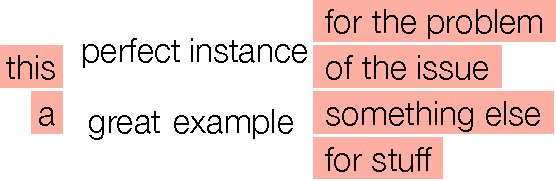
\includegraphics[width=0.99\linewidth]{figures/ngram_context.pdf}
\end{center}
\caption{An example of immediate lexical context acquisition over
  n-gram corpora. Left- and right-adjacent unigrams are stored as
  features for the phrase. Here, ``perfect instance'' and ``great
  example'' share a number of contexts and would thus be assumed to be
  paraphrases.}\label{fig-ngram-context}
\end{figure}


\section{Evaluation Results}
\label{sec-results}

To rate the quality of our output, we solicit human judgments of the
compressions along two five-point scales: grammaticality and
meaning. Judges are instructed to decide how much the meaning from a
reference translation is retained in the compressed sentence, with a
score of 5 indicating that all of the important information is
present, and 1 being that the compression does not retain any of the
original meaning. Similarly, a grammar score of 5 indicates perfect
grammaticality, and a grammar score of 1 is assigned to sentences that
are entirely ungrammatical. It is known that evaluation quality
correlates linearly with compression rate \cite{Napoles2011}. Thus, to
ensure fairness in comparing our systems, we adjust compression rates
to closely match on the sentence-level.

In Table~\ref{human_judgments} we compare our distributional
similarity-augmented paraphraser to the plain pivoting baseline and
the ILP approach at a compression rate of $\approx 0.79$. We can see
that the paraphrase approach significantly outperforms ILP on meaning
retention. However it shows notable weaknesses in
grammaticality. Adding $n$-gram-based distributional similarity
information to the paraphrases recovers some of the difference in
grammaticality and also yields gain in the compressions' meaning
retention. Moving to the rich distributional signatures yields
additional improvement.

Figure~\ref{num-ties-wins} shows a pairwise comparison breakdown
detailing the number of wins and ties in the human judgements for each
comparison. As suggested by our analysis in Section~\ref{sec-ranking},
there is substantial overlap between the baseline system and the
$n$-gram distributional similarity model, while the rich feature set
leads to noticeably different output far more often. The meaning
retention improvements over both the baseline and ILP are
statistically significant at $p < 0.05$.

\begin{figure}[!t]
\begin{center}
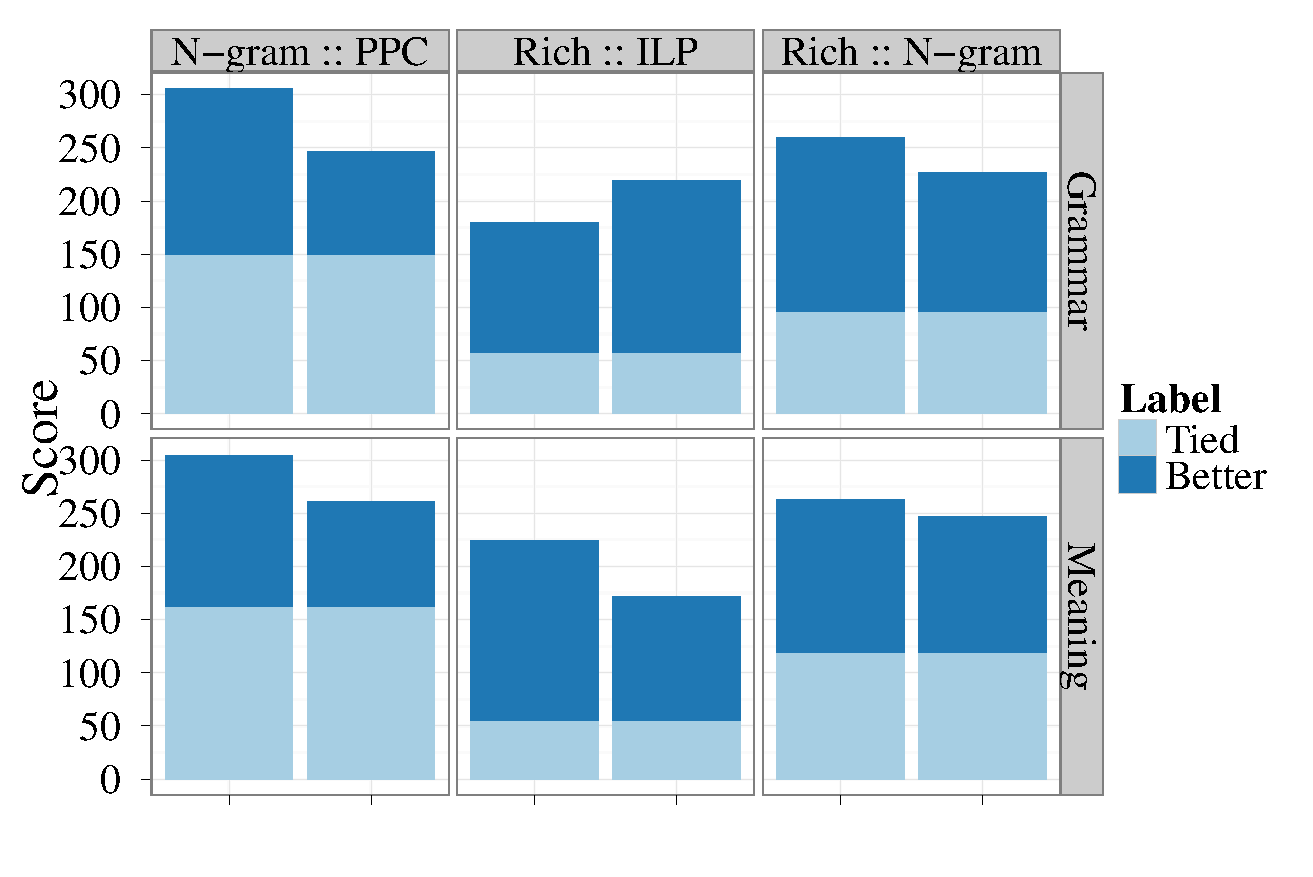
\includegraphics[width=0.99\linewidth]{figures/pairwise_comparison.pdf}
\end{center}
\caption{A pairwise breakdown of the human judgments comparing
  the systems. Light bleu regions show the number of times the twi systems were tied, and dark blue shows how many times one system was judged to be better than the other.}\label{num-ties-wins}
\end{figure}

Table~\ref{test_examples} shows an example sentence drawn from our
test set and the compressions produced by the different systems. We
see that both the paraphrase and ILP systems produce good quality
results, with the paraphrase system retaining the meaning of the
source sentence more accurately.

 \begin{table}
   \small
   \begin{center}
     \begin{tabular}{|c|c|c|c|}
       \hline
       & CR & Meaning & Grammar \\
       \hline
       Reference & 0.80 &  4.80 & 4.54 \\
       \hline
       ILP & 0.74 & 3.44 & {\bf 3.41} \\
       \hline
       \hline
       PC & 0.78 & 3.53 & 2.98 \\
       \hline
       PC + $n$-gram & 0.80 & 3.65 & 3.16 \\
       PC  + rich features & 0.79 & {\bf 3.70} & 3.26 \\
       \hline
       \hline
       Random Deletions & 0.78 & 2.91 & 2.53 \\
       \hline
     \end{tabular}
   \end{center}
   \normalsize
   \caption{Results of the human evaluation on longer compressions:
     pairwise compression rates (CR), meaning and grammaticality scores. 
     Bold indicates a statistically significance difference at $p <
     0.05$.}
   \label{human_judgments}
 \end{table}


\begin{table*}[!th]
\begin{center}
\small
{
\renewcommand{\arraystretch}{1.5}
\begin{tabular}{|c|>{\raggedright}m{13.2cm}|}
%  \hline
%  & \multicolumn{1}{|c|}{Sentences}  \\
  \hline

  Source & should these political developments have an impact on sports
  ? \tabularnewline
  \hline
  Reference & should these political events affect sports ? \tabularnewline
  \hline
  Rich & should these events have an impact on sports ? \tabularnewline
  \hline
  $n$-gram & these political developments impact on sports ? \tabularnewline
  \hline
  PC & should these events impact on sports ? \tabularnewline
  \hline
  ILP & political developments have an impact \tabularnewline
  \hline
  \hline

  Source & now we have to think and make a decision about our direction
  and choose only one way . thanks . \tabularnewline
  \hline
  Reference & we should ponder it and decide our path and follow it , thanks
  . \tabularnewline
  \hline
  Rich & now we think and decide on our way and choose one way . thanks
  . \tabularnewline
  \hline
  $n$-gram & now we have and decide on our way and choose one way . thanks
  . \tabularnewline
  \hline
  PC & now we have and decide on our way and choose one way . thanks
  . \tabularnewline
  \hline
  ILP &  we have to think and make a decision and choose way thanks
  \tabularnewline
  \hline
  \hline

  Source &  we are not poor . in fact , in our country , we are rich , and
  our poverty is in the lack of patriotism by some of the officials
  among us . \tabularnewline
  \hline
  Reference &  we are not poor in our country ; we are rich . our poverty is
  in the lack of patriotism of some of our officials . \tabularnewline
  \hline
  Rich & we are not poor . in fact in our country we are rich , and our
  poverty is the lack of patriotism by some officials us
  . \tabularnewline
  \hline
  $n$-gram & we are poor . in fact , our country , we are rich and
  poverty is no patriotism by some officials us . \tabularnewline
  \hline
  PC & we are not poor . in fact , in our country rich , and poverty
  is no patriotism by some officials among us . \tabularnewline
  \hline
  ILP & we are not poor in fact in our country we are rich and our
  poverty is in lack by some of officials among us \tabularnewline
  \hline
\end{tabular}
}
\normalsize
\end{center}
\caption{Example compressions produced by our systems and the baselines
  Table~\ref{human_judgments} for three input sentences from our test
  data.}
\label{test_examples}
\end{table*}

\section{Conclusion}
\label{sec-conclusion}

We presented a method to incorporate monolingual distributional
similarity into linguistically informed sentential paraphrase
extracted from bilingual parallel data. We investigated both the
effect of varying the feature set used for determining the
distributional signatures of phrases and conclude that a richer
feature set, even with significantly lower coverage, seems to
noticeably improve paraphrase quality in ranking. We evaluated our
integrated paraphrases on a text-to-text generation task and show that
our method significantly improves meaning retention over both a strong
paraphrastic baseline and a specialized state-of-the-art system.

\bibliographystyle{naaclhlt2012}
\bibliography{monods_t2t}
\end{document}